\documentclass[a4paper, 11pt]{article}
\usepackage[utf8]{inputenc}
\usepackage[english]{babel}
\usepackage[utf8]{inputenc}
\usepackage[margin=3.cm]{geometry}
\usepackage{fancyhdr}

\usepackage[T1]{fontenc}
\usepackage{lmodern}

\usepackage{graphicx}
\graphicspath{ {images/} }
\usepackage{pdflscape}


\usepackage{array}

\usepackage{color,array}

\usepackage{float}
\usepackage[table,xcdraw]{xcolor}

\usepackage{multirow}
\usepackage{slashbox} % Defines \backslashbox{..}{..}
\usepackage{adjustbox}

%Includes "References" in the table of contents
\usepackage[nottoc]{tocbibind}

\usepackage{enumitem}
\setlist{nolistsep}

\fancypagestyle{plain}{%
  \renewcommand{\headrulewidth}{0pt}%
  \fancyhf{}%
  \fancyfoot[L]{\footnotesize Raymond Lochner}
  \fancyfoot[C]{\footnotesize October 2017 - Université libre de Bruxelles}%
  \fancyfoot[R]{\thepage}
}
\pagestyle{plain}

\date{\today}

\begin{document}

\begin{titlepage}
	\centering
	{\scshape\LARGE Université libre de Bruxelles \par}
	\vspace{1cm}
	{\scshape\Large INFO-F-409 - Learning Dynamics\par}
	\vspace{1.5cm}
	{\huge\bfseries {Assignment One\par}}
	\vspace{2cm}
	{\Large Raymond Lochner - 000443637\par}
	\vspace{0.5cm}
	{\Large raymond.lochner@ulb.ac.be}
	\vfill
	
	\tableofcontents

\vfill
% Bottom of the page
	{\large \today \par}
\end{titlepage}

\newpage

\section{The Hawk-Dove game}

The Hawk-Dove game was first formulated by John Maynard Smith and Georg Prince in 1973 \cite{MaynardSmith1973}. The aim of the game is to gain a better understanding of conflicts in the animal kingdom. It consits of two players \{Player One, Player Two\} who have each two actions \{Hawk, Dove\}.The resulting payoff matrix can bee seen in Table \ref{tab-HawkDoveOriginal} where:
\begin{itemize}
  \item V = fitness value of winning resources in fight
  \item D = fitness costs of injury
  \item T = fitness costs of wasting time
\end{itemize}

and we assume that V,D,T $\geq$ 0.

\begin{table}[H]
\centering
\caption{Hawk-Dove Payoff Matrix}
\label{tab-HawkDoveOriginal}
\begin{tabular}{cl|ll|ll|}
\multicolumn{1}{l}{}                             &                       & \multicolumn{4}{c|}{Player Two}                                             \\ \cline{3-6} 
\multicolumn{1}{l}{}                             &                       & \multicolumn{2}{c|}{Hawk}              & \multicolumn{2}{c|}{Dove}          \\ \hline
\multicolumn{1}{c|}{\multirow{4}{*}{Player One}} & \multirow{2}{*}{Hawk} &         & \multicolumn{1}{r|}{(V-D)/2} &       & \multicolumn{1}{r|}{0}     \\
\multicolumn{1}{c|}{}                            &                       & (V-D)/2 &                              & V     &                            \\ \cline{2-6} 
\multicolumn{1}{c|}{}                            & \multirow{2}{*}{Dove} &         & \multicolumn{1}{r|}{V}       &       & \multicolumn{1}{r|}{V/2-T} \\
\multicolumn{1}{c|}{}                            &                       & 0       &                              & V/2-T &                            \\ \hline
\end{tabular}
\end{table}

In a mixed strategy game, we consider each player performing his action with a certain probability \textit{p} or \textit{q}, which results in the following payoff matrix displayed in Table \ref{tab-HawkDoveMixedStrategy}.

\begin{table}[H]
\centering
\caption{Hawk-Dove Probability Payoff Matrix}
\label{tab-HawkDoveMixedStrategy}
\begin{tabular}{cl|ll|ll|}
\multicolumn{1}{l}{}                             &                                & \multicolumn{4}{c|}{Player Two}                                             \\ \cline{3-6} 
\multicolumn{1}{l}{}                             &                                & \multicolumn{2}{c|}{P(Hawk)=q}         & \multicolumn{2}{c|}{P(Dove)=(1-q)} \\ \hline
\multicolumn{1}{c|}{\multirow{4}{*}{Player One}} & \multirow{2}{*}{P(Hawk)=p}     &         & \multicolumn{1}{r|}{(V-D)/2} &       & \multicolumn{1}{r|}{0}     \\
\multicolumn{1}{c|}{}                            &                                & (V-D)/2 &                              & V     &                            \\ \cline{2-6} 
\multicolumn{1}{c|}{}                            & \multirow{2}{*}{P(Dove)=(1-p)} &         & \multicolumn{1}{r|}{V}       &       & \multicolumn{1}{r|}{V/2-T} \\
\multicolumn{1}{c|}{}                            &                                & 0       &                              & V/2-T &                            \\ \hline
\end{tabular}
\end{table}

With this table we are able to calculate the payoff of the actions Hawk and Dove for Player One:

Player One's expected payoff for the strategy Hawk(p) is:
\[ q \times \frac{V-D}{2} + (1-q) \times V \]

Player One's expected payoff for the strategy Dove(1-p) is:
\[ q \times 0 + (1-q) \times ( \frac{V}{2} - T) = (1-q) \times ( \frac{V}{2} - T) \]

To find the best response set of all mixed strategies, we need to set them equal:

\[ q \times \frac{V-D}{2} + (1-q) \times V = (1-q) \times ( \frac{V}{2} - T) \]

\[ \frac{qV}{2} - \frac{qD}{2} + V - qV = \frac{V}{2} - T - \frac{qV}{2} + qT \]

\[ - \frac{qD}{2} + V = \frac{V}{2} - T + qT \]

\[ \frac{V}{2} + T = \frac{qD}{2} + qT \]

\[ \frac{V}{2} + T = q( \frac{D}{2} + T) \]

\[ V + 2T = q( D + 2T) \]

\[ q = \frac{V + 2T}{D + 2T} \]



%%%%%%%%%%%%%%%%%%%%%%%%%%%%%%%%%%%%%%%%%%%%%%%%%%%%%%%%%%%%%%%%%%%%%%%%%
\newpage
\section{Which social dilemma?}

Player A is confronted with one of three social dilemma's - the corresponding payoff matrix is shown in tables \ref{table-PrisonnersDilemma}, \ref{table-Stag-Hunt} and \ref{table-SnowdriftGame}. The player has to decide whether to cooperate (C) or to defect (D) without knowing which game he is actually facing. Each dilemma has the same probability $1/3$ of being played. Opponent B knows the game.


\begin{table}[!htb]
    \begin{minipage}{.33\linewidth}
      \caption{Prisonners dilemma}
      \label{table-PrisonnersDilemma}
      \centering
\begin{tabular}{l|l|l|}
  & C & D \\ \hline
C & \backslashbox{2}{2} & \backslashbox{0}{5}  \\ \hline
D & \backslashbox{5}{0} & \backslashbox{1}{1}  \\ \hline
\end{tabular}
    \end{minipage}%
    \begin{minipage}{.33\linewidth}
      \centering
      \caption{Stag-Hunt game}
      \label{table-Stag-Hunt}
\begin{tabular}{l|l|l|}
  & C & D \\ \hline
C & \backslashbox{5}{5} & \backslashbox{0}{2}  \\ \hline
D & \backslashbox{2}{0} & \backslashbox{1}{1}  \\ \hline
\end{tabular}
    \end{minipage} 
    \begin{minipage}{.33\linewidth}
      \centering
        \caption{Snowdrift game}
        \label{table-SnowdriftGame}
\begin{tabular}{l|l|l|}
  & C & D \\ \hline
C & \backslashbox{2}{2} & \backslashbox{1}{5}  \\ \hline
D & \backslashbox{5}{1} & \backslashbox{0}{0}  \\ \hline
\end{tabular}
    \end{minipage} 
\end{table}

with this information we can calculate the expected payoff for player A for every possible strategy of Player B - Table \ref{table-expectedPayoffForA}.

\begin{table}[!htb]
\centering
\caption{Expected payoff for Player A}
\label{table-expectedPayoffForA}
\begin{tabular}{lc|c|c|c|c|c|c|c|c|}
\cline{3-10}
                                                & \multicolumn{1}{l|}{} & \multicolumn{8}{c|}{Player B}                                                \\ \cline{3-10} 
                                                &                       & (C,C,C) & (C,C,D) & (C,D,C) & (C,D,D) & (D,C,C) & (D,C,D) & (D,D,C & (D,D,D) \\ \hline
\multicolumn{1}{|l|}{\multirow{2}{*}{Player A}} & C                     & 9/3     & 8/3     & 4/3     & 3/3     & 7/3     & 6/3     & 2/3    & 1/3     \\ \cline{2-10} 
\multicolumn{1}{|l|}{}                          & D                     & 12/3    & 7/3     & 11/3    & 6/3     & 8/3     & 3/3     & 7/3    & 2/3     \\ \hline
\end{tabular}
\end{table}

From this table we can select the best response for Player A for each strategy of Player B - cells marked red in Table \ref{table-expectedPayoffForA-SelectedCells}.

\begin{table}[!htb]
\centering
\caption{Best responses for Player A}
\label{table-expectedPayoffForA-SelectedCells}
\begin{tabular}{lc|c|c|c|c|c|c|c|c|}
\cline{3-10}
                                                 & \multicolumn{1}{c|}{} & \multicolumn{8}{c|}{Player B}                                                                                                                                                                                                                                          \\ \cline{3-10} 
                                                 &                       & (C,C,C)                                             & (C,C,D)                     & (C,D,C)                      & (C,D,D)                     & (D,C,C)                     & (D,C,D)                     & (D,D,C                      & (D,D,D)                     \\ \hline
\multicolumn{1}{|l|}{}                           & C                     & 9/3                                                 & \cellcolor[HTML]{FE0000}8/3 & 4/3                          & 3/3                         & 7/3                         & \cellcolor[HTML]{FE0000}6/3 & 2/3                         & 1/3                         \\ \cline{2-10} 
\multicolumn{1}{|l|}{\multirow{-2}{*}{Player A}} & D                     & \cellcolor[HTML]{FE0000}{\color[HTML]{000000} 12/3} & 7/3                         & \cellcolor[HTML]{FE0000}11/3 & \cellcolor[HTML]{FE0000}6/3 & \cellcolor[HTML]{FE0000}8/3 & 3/3                         & \cellcolor[HTML]{FE0000}7/3 & \cellcolor[HTML]{FE0000}2/3 \\ \hline
\end{tabular}
\end{table}


Now we have to determine the best responses of Player B against Player A of the three different strategies - marked by green cells in Tables \ref{table-PrisonnersDilemmaPayoffB}, \ref{table-Stag-HuntPayoffB} and \ref{table-SnowdriftGamePayoffB}.

\begin{table}[!htb]
    \begin{minipage}{.33\linewidth}
      \caption{Prisonners dilemma}
      \label{table-PrisonnersDilemmaPayoffB}
      \centering
\begin{tabular}{l|l|l|}
\cline{2-3}
                        & C & D                         \\ \hline
\multicolumn{1}{|l|}{C} & 2 & \cellcolor[HTML]{9AFF99}5 \\ \hline
\multicolumn{1}{|l|}{D} & 0 & \cellcolor[HTML]{9AFF99}1 \\ \hline
\end{tabular}
    \end{minipage}%
    \begin{minipage}{.33\linewidth}
      \centering
      \caption{Stag-Hunt game}
      \label{table-Stag-HuntPayoffB}
\begin{tabular}{l|l|l|}
\cline{2-3}
                        & C                         & D                         \\ \hline
\multicolumn{1}{|l|}{C} & \cellcolor[HTML]{9AFF99}5 & 2                         \\ \hline
\multicolumn{1}{|l|}{D} & 0                         & \cellcolor[HTML]{9AFF99}1 \\ \hline
\end{tabular}
    \end{minipage} 
    \begin{minipage}{.33\linewidth}
      \centering
        \caption{Snowdrift game}
        \label{table-SnowdriftGamePayoffB}
\begin{tabular}{l|l|l|}
\cline{2-3}
                        & C                         & D                         \\ \hline
\multicolumn{1}{|l|}{C} & 2                         & \cellcolor[HTML]{9AFF99}5 \\ \hline
\multicolumn{1}{|l|}{D} & \cellcolor[HTML]{9AFF99}1 & 0                         \\ \hline
\end{tabular}
    \end{minipage} 
\end{table}


The pure strategy Nash Equilibria can now be determined by matching these results. We find two Nash Equilibria at \{C,(D,C,D)\} and \{D,(D,D,C)\}.



%%%%%%%%%%%%%%%%%%%%%%%%%%%%%%%%%%%%%%%%%%%%%%%%%%%%%%%%%%%%%%%%%%%%%%%%%
\newpage
\begin{landscape}
\section{Sequential truel}


This scenario considers three persons A,B and C, each of whom has a gun with a single bullet. If alive, each person may shoot at any surviving person. The order in which the scenario is played out is A, then B and then C. The probability that player \textit{i} hits their target is denoted by $p_i$ where $0\leq p_i\leq 1$. Every player wishes to optimize her probability of survival.
For this exercise we further assume that a player has to target another living player and is not allowed to miss a shoot consciously. The resulting diagram of this game is shown in Figure \ref{fig-SeqTrualDiag}.

\begin{figure}[h]
\caption{Sequential truel diagram}
\label{fig-SeqTrualDiag}
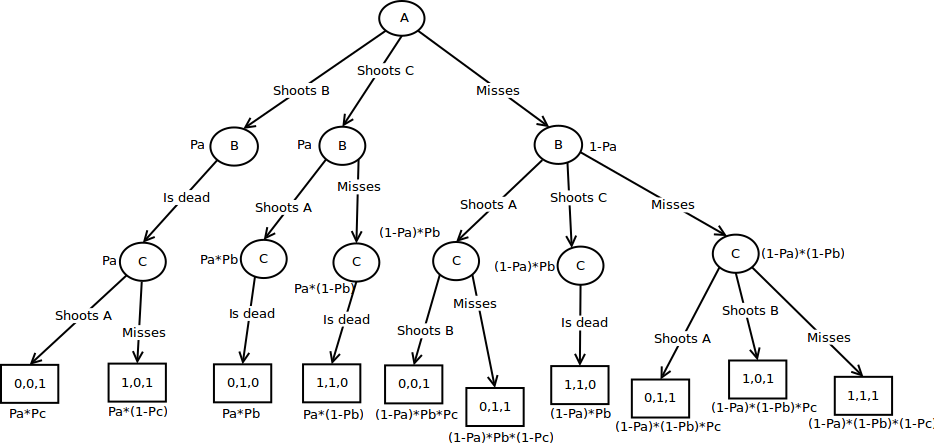
\includegraphics[scale=0.65]{SequentialTruelDiagram.png}
\end{figure}

\end{landscape}

The Diagram shows all possible actions of all players with all possible outcomes. The lowest level leaf indicates which player is still alive and with which probability - [0,0,1] indicates Player A and B being dead while Player C is alive with a probability of $p_a \times p_c$.

%%%%%%%%%%%%%%%%%%%%%%%%%%%%%%%%%%%%%%%%%%%%%%%%%%%%%%%%%%%%%%%%%%%%%%%%%
%% Bibliography start
\newpage

\bibliographystyle{unsrt}
\bibliography{bibliography}

\end{document}
